\section{拟采用的研究过程、技术路线、实验评估方案及其可行性分析}
本次研究的主要目的是借助TDD数据结构,构建能快速计算量子模型检测中可达问题的方案。因此主要采用的方法是模拟量子计算。本次研究的主要挑战在于尽可能减少程序的运行时间。为此,需要采用一系列方法来开发更有效的算法,以优化TDD操作和收缩张量网络。其中包括开发新技术来分割张量网络和优化TDD结构。在各种方法中,分割张量网络和拆分决策图被认为是主要的优化策略,并且已经取得了一定的研究成果。
\subsection{研究过程}
量子模型的跃迁系统定义为:$\mathcal{M}=\{\mathcal{H},Act,\{U_\alpha,\alpha\in Act\},\mathcal{H}_0\}$。以可达空间的研究过程为例,主要为以下几步:
\begin{myen}
	\item \label{item:process_inital}将可达空间初始化为$\mathcal{H}_0$。
	\item \label{item:process_state}取当前可达空间的最大纠缠态作为当前状态,并得到对应的TDD表示。
	\item \label{item:process_cir}获得量子电路,即转换关系$U_\alpha,\alpha\in Act$的TDD表示。
	\item \label{item:process_cont} 将前两步的TDD进行收缩,即通过基于TDD模拟计算得到下一个量子状态的TDD。
	\item \label{item:process_end}将下一个TDD加入到可达空间中,如果可达空间发生变化,回到\ref{item:process_state}步,否则结束。
\end{myen}
	
依据系统的可达空间,就可以对其他可达性问题进行分析。整个研究过程也基本按实现过程逐步推进。
\subsection{技术路线}
在应用TDD计算模型检测中,存在两个关键步骤。第一步是获取量子线路的TDD表示。第二步是逐步收缩表示当前状态的TDD与表示量子线路的TDD,最终得到下一步状态的TDD。在这两个步骤中加入好的优化方法是能够减少运行时间的关键。在不同的分割量子线路方案中,有两类主要技术路线,下文将简要介绍。除了拆分方案以外,优化TDD结构也是一种思路。
\subsubsection{addition的拆分方案}
\label{addition}
第一种被称为addition\citep{chen2018classical}。将量子电路视为张量网络,首先将一个量子电路C转换成无向图G。G中的每个节点表示量子电路的一个索引,并且如果它们是相同门的输入或输出索引,则在G中连接两个节点。并且当满足以下两个条件之一时输入和输出索引不变:
\begin{itemize}
	\item 是对角线量子门的输入和输出索引;
	\item 是受控门的控制比特位的输入和输出索引。
\end{itemize}
	
该图描述了量子电路的连通性,通过选择图中连通度最大的索引可以对电路进行分割。图\ref{fig:addition}展示了Grover\_3电路图的索引链接图。因此选择图中连通度较大的$x_1^1,x_1^3x_2^1$可以对电路进行较好的划分。
 
\begin{figure}[!htbp]
	\centering
	\includegraphics[height=5cm]{Img/cir_index_graph.pdf}
	\caption{Grover\_3的索引连接图}
	\label{fig:addition}
\end{figure} 
\subsubsection{contraction的拆分方案}\label{contraction}
另一种方法成为contraction。在这一方法中,将量子电路划分为若干个较小的部分,其收缩等于原始电路。对于两个预设整数参数k1和k2,将电路划分为若干小电路。其中每个小电路涉及最多k1个量子比特,并且与至多跨越不同部件的k2个多比特门相连。图\ref{fig:contraction}展示了对Bit flip电路进行k1=3,k2=2的拆分结果。
\begin{figure}[!htbp]
	\centering
	\includegraphics[height=5cm]{Img/cir_contraction.pdf}
	\caption{对量子电路进行contraction的拆分}
	\label{fig:contraction}
\end{figure} 
\subsubsection{优化TDD结构}

在BDD中,索引的顺序很重要。因为索引顺序会直接影响BDD的大小。一个良好的变量顺序可以使得BDD比一个糟糕的变量顺序小得多。图\ref{fig:bdd-compare}的了两张图都表示了布尔函数ƒ(x1,...,x8)=x1x2+x3x4+x5x6+x7x8,但图\ref{fig:bdd-good}的结构更简单。其中图\ref{fig:bdd-bad}的索引顺序为\{x1,x3,x5,x7,x2,x4,x6,x8\},图\ref{fig:bdd-good}的索引顺序为\{x1,x2,x3,x4,x5,x6,x7,x8\}。找到一个好的索引顺序是一个NP问题,在具体使用中,只能避免最差的情况,并尽量使用使结构最简的索引顺序。

\begin{figure}[!htbp]
	\centering
	\begin{subfigure}[b]{.4\textwidth}
        \centering
        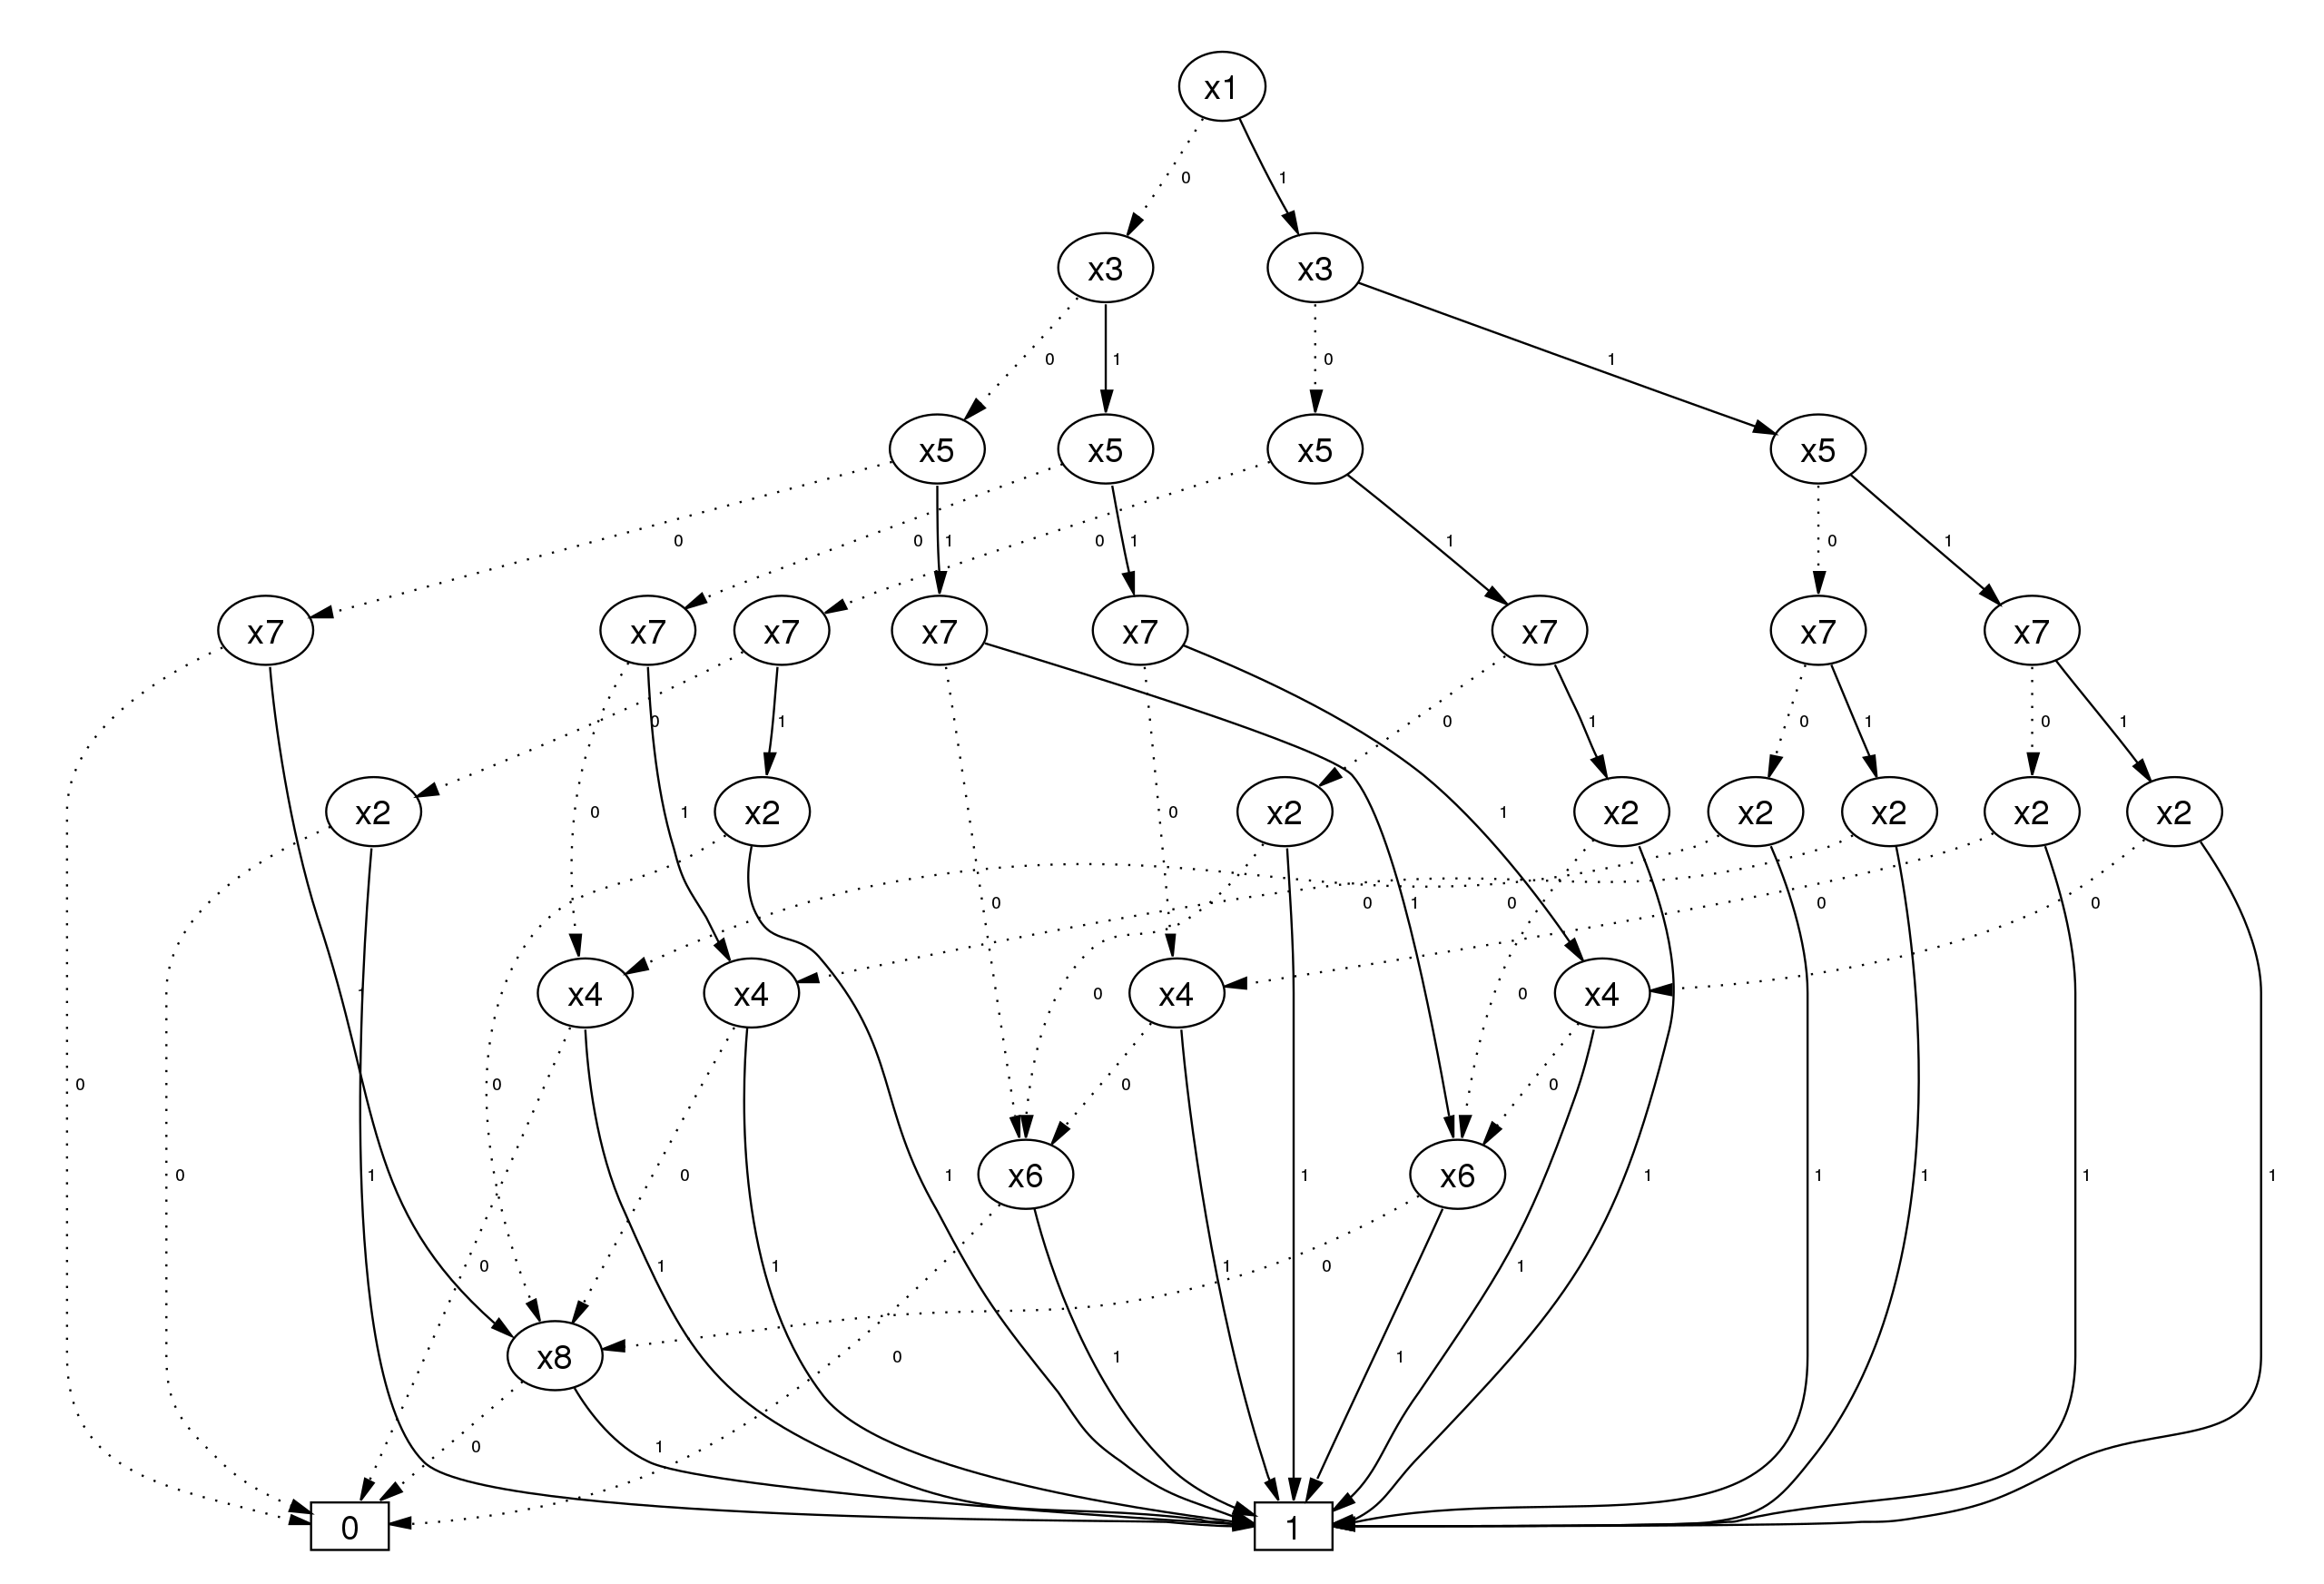
\includegraphics[height=5cm]{Img/BDD_Variable_Ordering_Bad.svg.pdf}
		\caption{索引顺序为\{x1,x3,x5,x7,x2,x4,x6,x8\}}
		\label{fig:bdd-bad}
	\end{subfigure}
	\begin{subfigure}[b]{.4\textwidth}
        \centering
        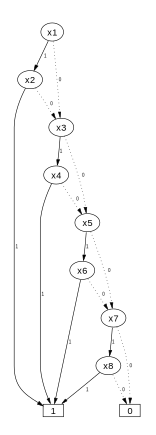
\includegraphics[height=5cm]{Img/BDD_Variable_Ordering_Good.svg.pdf}
		\caption{索引顺序为\{x1,x2,x3,x4,x5,x6,x7,x8\}}
		\label{fig:bdd-good}
	\end{subfigure}
	\caption{同一布尔函数在不同索引顺序下的结构图\citep{wiki:bdd}}
	\label{fig:bdd-compare}
\end{figure}

TDD与BDD类似,也有索引顺序问题。在工程实现中,尽量使用能简化TDD结构的索引顺序也是能降低计算时间的一种技术路线。
% //TODO: 增加limdd
\subsection{实验评估方案}
本次研究的主要关注点是时间效率。为了确保研究工作的实用性,在完成研究后需要对计算过程的时间消耗进行评估。为此,将借助不同的量子算法来进行综合评估。在评估过程中,需要选择目前已经被广泛应用和验证的量子算法,如Grover算法、BV算法和QRW算法等。从而保证研究项目的实用性。
通过评估时间效率,可以对研究成果进行客观的评估和比较。此外,为了更好地了解研究成果在当前领域中的地位,还需要与其他相关研究成果进行对比。例如,与基于QMDD的研究和使用TensorFlow等工具的研究进行比较。通过与这些类似研究成果的对比,可以更全面地评估研究成果在时间效率方面的优势和差距。
这样的评估和对比分析将,可以为研究工作提供更多的参考和支持。通过与其他方法的对比,可以更好地理解我们的方法在量子模型检测中的优势和局限性,并为进一步的研究和实际应用提供指导。
\subsection{可行性分析}
首先,本项目在前期已进行了较为充分的文献资料搜集和调研工作,对目前量子模型检测技术现状、相关工作、现有项目的优缺点、验证需求有较为充分的认识,为后期的研究和实验工作打下了坚实的基础。
其次电路拆分方案是最直接降低运行时间的一类方案。而前期已经小范围尝试该方案的时间效率。表\ref{table:split}展示了计算不同测试image computation,应用不同拆分方案的用时。其中basic表示没有使用优化技术,addition表示使用addition优化技术,contraction表示使用contraction优化技术,时间单位为秒。

\begin{table}[!htbp]
	\centering
	\begin{tabular}{@{}llll@{}}
	\toprule
	Benchmark  & basic   & addition & contraction \\ \midrule
	Grover\_20 & 294.65  & 259.87   & 4.39        \\
	QFT\_20    & 1199.21 & 655.19   & 0.12        \\
	QRW\_20    & 341.05  & 218.29   & 14.31       \\
	BV\_100    & 7.36    & 7.43     & 0.41        \\ \bottomrule
	\end{tabular}
	\caption{不同拆分方案在不同类型测试中用时}
	\label{table:split}
\end{table}

